\documentclass[10pt,conference,onecolumn]{IEEEtran}

\usepackage[utf8]{inputenc}
\usepackage[T1]{fontenc}
\usepackage{graphicx}
\usepackage{booktabs}
\usepackage{multirow}
\usepackage{amsmath}
\usepackage{amssymb}
\usepackage{hyperref}
\usepackage{url}
\usepackage{xcolor}
\usepackage{array}
\usepackage{tikz}
\usetikzlibrary{arrows.meta,positioning,shapes.geometric}

\title{Kolmogorov-Arnold Networks for Forecasting:\\
An Interpretable Comparative Study on Climate and Electricity Data}

\author{
\IEEEauthorblockN{Kirill Alekhin}
\IEEEauthorblockA{
ITMO University\\
Saint Petersburg, Russia\\
\texttt{alekkhin.kirill.list.ru}
}
}

\begin{document}

\maketitle

\begin{abstract}
This paper presents an extended empirical study of Kolmogorov-Arnold Networks (KAN) and hybrid KAN architectures in forecasting tasks with markedly different structure, data-generating mechanisms, and practical constraints. The first case study addresses multivariate climate time series forecasting on the UCI Air Quality dataset, where KAN-based models are compared with recurrent and feed-forward neural baselines in both standard and robustness-oriented regimes. The second case study focuses on short-term electricity price forecasting on a leakage-safe panel dataset constructed from Russian regional energy market data, where the learning problem is complicated by mixed-frequency inputs, regional heterogeneity, and strict causal alignment requirements. In the baseline electricity setup, strong tabular models outperform direct KAN formulations by a substantial margin. However, after reformulating the target as a next-step price increment, incorporating region embeddings, and introducing residual learning, the strongest KAN-based model approaches the performance of the best boosting baseline much more closely. Across both case studies, the experiments show that the main value of KAN is not universal predictive dominance, but the combination of nonlinear modeling flexibility, architectural modularity, and interpretability through learned channel-wise $\phi$-functions. The paper therefore contributes not only a benchmark-style comparison, but also a problem-design perspective: KAN is most useful when the forecasting task is formulated in a way that matches its inductive bias and when interpretability is treated as a first-class modeling objective rather than as an afterthought.
\end{abstract}

\begin{IEEEkeywords}
Kolmogorov-Arnold Networks, forecasting, time series, panel data, electricity price, climate data, interpretability, hybrid neural models
\end{IEEEkeywords}

\section{Introduction}

Forecasting is one of the central tasks in applied machine learning and data mining. In practice, forecasting models are used to support operational planning in climate science, industrial systems, electricity markets, logistics, finance, and many other domains. The quality of forecasts affects decision making directly, which means that model errors can translate into operational, economic, or even safety-related risks. For this reason, modern forecasting research increasingly focuses not only on predictive accuracy, but also on stability, robustness, and interpretability.

Real-world forecasting tasks are difficult for at least three reasons. First, the observed dynamics are often nonlinear and partially nonstationary. Second, the available data may contain missing values, noise, duplicated signals, and heterogeneous feature types. Third, the forecasting objective itself can vary significantly: some tasks are essentially multivariate sequence modeling, while others are better seen as panel or tabular prediction with temporal dependencies. This diversity makes it unlikely that a single model family will dominate in all scenarios.

Recently, Kolmogorov-Arnold Networks (KAN) have emerged as a promising alternative to traditional multilayer perceptrons \cite{liu2024kan}. The key architectural idea of KAN is to learn one-dimensional nonlinear transformations on connections rather than relying only on fixed activations applied to hidden node outputs. This makes KAN interesting for forecasting for two reasons. On the one hand, it offers a flexible way to model nonlinear dependencies. On the other hand, it introduces a potentially interpretable representation through learned $\phi$-functions, which can be visualized and analyzed channel by channel.

Despite this promise, the role of KAN in practical forecasting remains insufficiently understood. Existing discussions often focus on benchmark or synthetic settings, while applied forecasting tasks involve substantially more constraints: leakage from future information, strong seasonal structure, panel heterogeneity, and the need to compare not only with neural baselines but also with strong non-neural models such as gradient boosting and linear regression.

This paper is motivated by the following research question: \emph{under what conditions can KAN and hybrid KAN architectures serve as effective and interpretable forecasting models on real data?} To answer this question, we investigate two forecasting problems with very different structure:
\begin{itemize}
    \item a multivariate climate time series forecasting task based on the UCI Air Quality dataset;
    \item a short-term electricity price forecasting task on Russian regional energy market data, formulated as a leakage-safe panel forecasting problem.
\end{itemize}

The first case study is useful because it provides a relatively clean multivariate sequence modeling setup, where KAN can be compared directly with LSTM and MLP models and where $\phi$-functions are easy to interpret. The second case study is substantially harder and more realistic: it combines hourly, daily, and monthly information, exhibits strong regional heterogeneity, and requires careful handling of leakage from future information.

The broader motivation behind using these two cases together is methodological rather than merely illustrative. A single benchmark can only show whether a model works well in one environment; it cannot reveal how strongly that performance depends on problem structure. By contrast, the joint climate--electricity design allows us to examine where KAN is naturally aligned with the data and where it needs architectural or target-level adaptation. In other words, the paper does not ask only whether KAN works, but also \emph{why} it works better in some forecasting regimes than in others.

This distinction is particularly important for applied machine learning. In real projects, practitioners rarely choose between models in a vacuum. They choose between modeling pipelines that differ in feature engineering burden, robustness to missing values, compatibility with domain knowledge, and interpretability for downstream users. A model that is slightly weaker in raw predictive accuracy may still be preferable if it offers a much clearer explanation of which feature groups and nonlinear effects drive the forecast. This is especially relevant in scientific and energy applications, where results are often communicated to stakeholders who need to audit the reasoning behind a prediction rather than simply consume a single scalar output.

The contributions of the paper are the following:
\begin{itemize}
    \item We provide a comparative KAN study on two applied forecasting domains with different structural properties.
    \item We construct a leakage-safe electricity forecasting dataset from Russian regional energy data and evaluate KAN-based and non-KAN baselines on it.
    \item We show that a naive KAN formulation is insufficient for the electricity task, but that target reformulation, region embeddings, and residual learning substantially improve KAN performance.
    \item We analyze KAN interpretability through $\phi$-functions, channel contributions, and grouped feature importance.
    \item We discuss the conditions under which KAN is most useful as a forecasting model and as an interpretable nonlinear analysis tool.
\end{itemize}

The rest of the paper is organized as follows. Section II reviews the theoretical and empirical background on KAN, forecasting baselines, and interpretability. Section III introduces the methodological setup, model families, and evaluation logic. Sections IV and V present the climate and electricity case studies, respectively. Section VI synthesizes the findings across both domains, Section VII discusses threats to validity, and Section VIII concludes with practical implications and directions for future work.

\section{Related Work}

\subsection{Kolmogorov-Arnold Representation and KAN}

The theoretical motivation of KAN stems from the Kolmogorov-Arnold representation theorem \cite{kolmogorov1957,arnold1963}, which states that multivariate continuous functions can be represented through superpositions of one-dimensional functions. This result has long been interpreted as a theoretical basis for constructing function approximation schemes with explicit one-dimensional nonlinear components.

Modern KAN architectures translate this principle into neural computation by replacing part of the traditional node-centric nonlinear processing with learned nonlinear edge transformations \cite{liu2024kan}. Instead of applying a fixed nonlinearity such as ReLU after a linear layer, KAN learns a family of basis-weighted one-dimensional functions that can approximate different forms of nonlinear input-output dependence.

\subsection{Forecasting Architectures}

For time series forecasting, recurrent and sequence models remain important baselines. LSTM networks are still widely used as strong recurrent baselines for multivariate temporal prediction, especially in moderate-sized settings where interpretability is not the primary goal. Transformer-based models have also become prominent in long-horizon forecasting \cite{zhou2021informer}, but in many applied scenarios simpler baselines remain difficult to outperform consistently.

In contrast, for tabular or panel forecasting tasks, tree-based ensembles and regularized linear models are often extremely competitive. Gradient boosting models are particularly strong when the data contain mixed-scale signals, nonlinear interactions, and moderate amounts of engineered lag and calendar features. Therefore, any applied claim about KAN must be evaluated not only against neural baselines such as LSTM or MLP, but also against strong tabular baselines.

The continued relevance of LSTM models in forecasting is well established in sequence modeling literature \cite{hochreiter1997lstm}. At the same time, the success of gradient boosting for tabular machine learning is equally well documented \cite{friedman2001greedy,prokhorenkova2018catboost}. This duality matters for our paper: the climate task is close to the type of problem where recurrent or neural sequence models are natural, whereas the electricity task contains enough engineered structure that strong tabular methods should be treated as first-class competitors rather than auxiliary baselines.

\subsection{Interpretability in Forecasting}

Interpretability is a major challenge in forecasting. Standard deep sequence models often act as black boxes, making it difficult to understand which variables, lags, or temporal regimes are driving predictions. One of the attractive aspects of KAN is that it naturally exposes nonlinear channel-wise transformations via learned $\phi$-functions. This does not make all KAN models fully transparent, but it provides a more structured interpretability mechanism than purely latent representations.

Interpretability is especially important in applied energy systems, where model outputs may be used for dispatch, cost planning, and market-oriented decision support. In such settings, a small gain in accuracy does not automatically dominate a model that is slightly less accurate but easier to audit, debug, and communicate to domain experts. This is one of the central practical motivations behind our comparative study.

\section{Methodology}

\subsection{Problem Formulation}

We consider supervised forecasting under two related but distinct formulations.

\textbf{Multivariate time series forecasting.} Given a sequence window
\begin{equation}
X_t = [x_{t-w+1}, \dots, x_t],
\end{equation}
where each $x_t \in \mathbb{R}^d$, the task is to predict either the next step or a multi-step horizon
\begin{equation}
Y_t = [x_{t+1}, \dots, x_{t+h}].
\end{equation}

\textbf{Panel forecasting.} Given observations indexed by time and region, the task is to predict a region-specific target at $t+1$ using lagged values, calendar information, and region-level attributes. This setup combines time dependence with cross-sectional heterogeneity.

These two formulations were intentionally selected to stress different inductive biases. The multivariate climate task emphasizes temporal coherence and cross-channel dependencies inside a single evolving process. The electricity task emphasizes heterogeneous entities, mixed-frequency predictors, and the need to preserve causality under realistic data availability constraints.

From a modeling perspective, these two formulations imply different notions of difficulty. In the climate task, the main challenge is to learn a compact nonlinear representation of coupled sensor trajectories over time. In the electricity task, the challenge is broader: the model must combine lagged dynamics with entity-specific structure, calendar regularities, and slowly varying exogenous variables while avoiding spurious information flow from the future. This makes the second task less similar to a pure sequence benchmark and more similar to structured industrial forecasting, where data preparation and target definition often determine model quality as much as the learning architecture itself.

\subsection{Model Families}

We evaluate the following model families:
\begin{itemize}
    \item \textbf{KAN}: a two-layer KAN model using basis-weighted nonlinear transformations;
    \item \textbf{Hybrid KAN}: a linear branch plus a nonlinear KAN branch;
    \item \textbf{KANEmbedDelta}: a KAN model trained on the next-step price increment and augmented with region embeddings;
    \item \textbf{HybridKANEmbedDelta}: a strengthened hybrid KAN using region embeddings and a delta target;
    \item \textbf{ResidualRidgeKAN}: a residual-learning setup where Ridge predicts the main signal and KAN predicts the residual component;
    \item \textbf{LSTM}, \textbf{MLP}: neural baselines for climate forecasting;
    \item \textbf{Linear Regression}, \textbf{Ridge}, \textbf{HistGradientBoosting}: strong baselines for the electricity case.
\end{itemize}

For hybrid KAN models, the forecast is represented as
\begin{equation}
\hat{y} = f_{\text{linear}}(x) + f_{\text{KAN}}(x).
\end{equation}
This decomposition is useful because it allows the model to explain simple global effects through the linear branch and to capture structured nonlinearities through the KAN branch.

In the strengthened electricity setup, the residual model can also be written as
\begin{equation}
\hat{y} = f_{\text{Ridge}}(x) + f_{\text{KAN}}(x),
\end{equation}
where the second term is trained on residual targets. Conceptually, this setup shifts KAN from full-response modeling to targeted nonlinear correction.

This distinction is conceptually important. A direct predictor must learn all components of the forecasting signal simultaneously: global trend, local dynamics, region-specific effects, and residual nonlinearities. A residual KAN model is much more specialized. It can leave simple and approximately linear structure to a strong baseline model and concentrate its representational capacity on the part of the signal that is hardest to capture with conventional methods. In forecasting applications with heterogeneous feature groups, this division of labor can be more effective than forcing a single model family to explain everything at once.

\begin{figure}[t]
\centering
\resizebox{0.95\textwidth}{!}{%
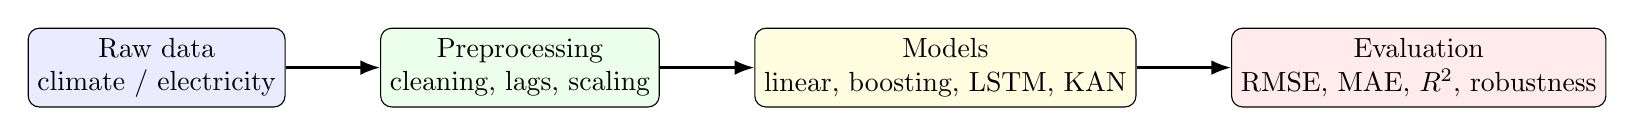
\begin{tikzpicture}[
node distance=1.2cm,
box/.style={draw, rounded corners, align=center, minimum width=2.7cm, minimum height=1cm},
arr/.style={-{Latex[length=2.5mm]}, thick}
]
\node[box, fill=blue!8] (data) {Raw data\\ climate / electricity};
\node[box, fill=green!8, right=of data] (prep) {Preprocessing\\ cleaning, lags, scaling};
\node[box, fill=yellow!12, right=of prep] (models) {Models\\ linear, boosting, LSTM, KAN};
\node[box, fill=red!8, right=of models] (eval) {Evaluation\\ RMSE, MAE, $R^2$, robustness};
\draw[arr] (data) -- (prep);
\draw[arr] (prep) -- (models);
\draw[arr] (models) -- (eval);
\end{tikzpicture}
}
\caption{Overall workflow of the comparative study across both forecasting domains.}
\label{fig:workflow}
\end{figure}

\subsection{Implementation Notes}

The experiments were implemented in Python using NumPy, pandas, scikit-learn, PyTorch, and Jupyter notebooks for exploratory analysis. For the electricity task, the workflow was organized as a reproducible pipeline with separate stages for panel construction, leakage-safe feature alignment, model training, metric calculation, and interpretability output generation.

The KAN-based models were implemented as compact research prototypes rather than as direct wrappers around a third-party benchmark suite. This was necessary because the study required explicit control over leakage-safe temporal alignment, region embedding logic, and extraction of interpretable intermediate artifacts such as learned $\phi$-functions and grouped channel contributions.

This implementation strategy also improves scientific transparency. Rather than optimizing only for benchmark throughput, the project was organized to preserve visibility into each stage of the pipeline: how samples were constructed, how targets were shifted, how region information entered the model, and how interpretability artifacts were saved. For research writing and thesis presentation, such transparency is often more valuable than a narrowly optimized training script, because it allows the full modeling logic to be inspected and defended.

\subsection{Interpretability Framework}

We use four complementary interpretability mechanisms:
\begin{itemize}
    \item visualization of learned $\phi$-functions in the first KAN layer;
    \item feature importance derived from KAN coefficients or activation-based contributions;
    \item grouped permutation importance for meaningful feature channels;
    \item qualitative inspection of predicted versus observed trajectories.
\end{itemize}

For pure KAN, interpretation is relatively direct because the model consists mostly of nonlinear channel-wise transformations. For hybrid KAN, interpretability becomes partial rather than absolute, since the final forecast combines linear and nonlinear components. We therefore interpret hybrid models as \emph{partially interpretable} rather than fully transparent.

In practice, this interpretability framework answers three distinct questions. First, \emph{which feature groups matter most}? This is addressed by grouped permutation or contribution analysis. Second, \emph{how do important variables affect the response}? This is addressed by the shapes of learned $\phi$-functions. Third, \emph{does the model behave plausibly at the trajectory level}? This is addressed by visually comparing predictions and observations across representative temporal segments. Taken together, these views provide a richer understanding than a single global importance ranking.

\subsection{Evaluation Metrics}

We use the following metrics:
\begin{itemize}
    \item RMSE for overall predictive deviation;
    \item MAE for average absolute error;
    \item $R^2$ for explained variance;
    \item qualitative robustness comparisons under noise, missingness, and reduced sample size in the climate case.
\end{itemize}

RMSE is emphasized in the main discussion because it penalizes large errors more strongly and therefore better reflects the cost of unstable forecasts in many real settings. MAE is included because it is easier to interpret in the original target scale, while $R^2$ provides a normalized summary of how much variance is captured by the model.

We do not claim that these metrics exhaust all practically relevant criteria. In energy applications, directional accuracy, peak-event prediction, or asymmetric cost measures may also be important. Nevertheless, RMSE, MAE, and $R^2$ provide a sufficiently informative common basis for comparing diverse model families across both case studies without introducing task-specific metrics that would weaken cross-domain comparability.

\section{Case Study I: Climate Forecasting}

\subsection{Dataset}

The climate case study uses the UCI Air Quality dataset \cite{devito2008airquality}. After cleaning and removing invalid placeholders, we focus on the following five variables:
\begin{itemize}
    \item CO(GT);
    \item NO$_2$(GT);
    \item C$_6$H$_6$(GT);
    \item temperature;
    \item relative humidity.
\end{itemize}

These variables form a multivariate temporal process with both chemical and meteorological structure. The data are standardized, and sliding windows are used to construct train/test splits without shuffling, preserving temporal order.

The climate case is deliberately useful as a ``controlled'' forecasting environment. Although it is a real dataset rather than a synthetic benchmark, it is still much cleaner than the electricity panel. The variables interact within a single temporal system, the feature semantics are easy to explain, and the target construction is straightforward. This makes the case study well suited for isolating the modeling behavior of KAN and hybrid KAN without immediately entangling the analysis with entity embeddings, leakage-safe joins across frequencies, or highly irregular operational covariates.

\subsection{Preprocessing}

The climate dataset required several preprocessing steps before modeling. First, invalid placeholders representing missing sensor measurements were removed or converted to proper missing values. Second, the selected variables were aligned in time and standardized. Third, forecasting samples were created with sliding windows so that each training example contained a fixed-length history and a future prediction target.

This preprocessing is relatively conventional, but it is important for fair comparison. Without a consistent windowing strategy, the performance of sequence models such as LSTM and KAN would not be directly comparable.

An additional reason this preprocessing matters is interpretability. When all variables are standardized and aligned consistently, the learned nonlinear transformations can be compared more meaningfully across channels. Otherwise, visually large nonlinear effects could simply reflect different raw scales rather than genuine differences in functional dependence. Because one of the paper's goals is to inspect learned $\phi$-functions rather than merely report final metrics, disciplined preprocessing is not just a technical necessity but part of the interpretability design.

\subsection{Experimental Setup}

The climate experiments include:
\begin{itemize}
    \item standard forecasting on the full dataset;
    \item forecasting with artificially injected missing values;
    \item forecasting with additive noise;
    \item forecasting with a reduced training set.
\end{itemize}

This design allows us to evaluate not only pointwise predictive quality but also robustness to data degradation, which is important for practical forecasting systems.

The climate case therefore serves two purposes in the overall paper. It is not only a benchmark where KAN can be tested under favorable sequence conditions, but also a controlled environment for analyzing the qualitative behavior of learned nonlinear transformations.

In other words, the climate experiments help answer a foundational question before we move to the more difficult electricity case: if KAN is given a setting that is structurally compatible with its design, does it actually exhibit the advantages often claimed in the literature? The robustness scenarios help prevent an overly optimistic answer based only on clean-data performance. A model that performs well only in an idealized regime is far less interesting for applied forecasting than one that remains stable when observations are noisy, incomplete, or limited in quantity.

\subsection{Results on the Full Dataset}

Table~\ref{tab:climate_main} summarizes the main results on the climate forecasting task.

\begin{table}[t]
\centering
\caption{Climate forecasting results on the full dataset}
\label{tab:climate_main}
\begin{tabular}{lccc}
\toprule
Model & RMSE & MAE & $R^2$ \\
\midrule
Hybrid KAN & 0.881 & 0.696 & 0.344 \\
LSTM & 0.923 & 0.726 & 0.281 \\
MLP & 0.998 & 0.793 & 0.158 \\
KAN & 1.014 & 0.799 & 0.132 \\
\bottomrule
\end{tabular}
\end{table}

Hybrid KAN achieved the best RMSE among the tested neural architectures. This suggests that, for a multivariate sequence forecasting task with moderate dimensionality, combining a direct linear path with KAN-based nonlinear feature transformations is beneficial.

The result is notable not simply because Hybrid KAN ranks first, but because of the way it wins. The margin over LSTM is meaningful yet not extreme, which suggests that KAN is not exploiting some accidental peculiarity of the dataset. Instead, the evidence points to a more general pattern: a hybrid architecture can separate relatively smooth linear tendencies from more structured nonlinear interactions. This is consistent with the idea that environmental sensor data contain both approximately linear co-movement and variable-specific nonlinearities, and that explicitly modeling both components can improve forecasting quality.

\subsection{Robustness Experiments}

Table~\ref{tab:climate_robust} reports RMSE under the robustness scenarios used in the climate experiments.

\begin{table}[t]
\centering
\caption{Climate forecasting robustness results (RMSE)}
\label{tab:climate_robust}
\begin{tabular}{lcccc}
\toprule
Model & Full & Missing & Noise & Small \\
\midrule
Hybrid KAN & 0.881 & 0.855 & 0.871 & 0.931 \\
KAN & 1.014 & 1.033 & 1.023 & 1.021 \\
LSTM & 0.923 & 0.919 & 0.943 & 0.930 \\
MLP & 0.998 & 0.948 & 0.988 & 0.943 \\
\bottomrule
\end{tabular}
\end{table}

The robustness results are important for two reasons. First, they show that the superiority of Hybrid KAN on the climate task is not limited to the clean full-data regime. Second, they support the idea that hybridization may stabilize KAN-style nonlinear transformations when the input signal is degraded.

The pattern across conditions is arguably more informative than the absolute scores. If a model remains near the top across missingness, noise, and smaller training subsets, this suggests that its inductive bias is not narrowly tuned to a single data regime. Such stability is especially relevant for sensor-driven applications, where measurement failures and short calibration intervals are common. From that perspective, Hybrid KAN appears not only accurate but also practically resilient.

\subsection{Interpretability on Climate Data}

The climate task is especially convenient for KAN interpretation. The learned $\phi$-functions can be visualized directly for selected input-output pairs, which helps reveal whether the model relies on monotonic, oscillatory, or saturating nonlinear transformations. In our experiments, the $\phi$-function plots showed that different output variables were associated with noticeably different input-response patterns, indicating that the network was not simply learning a generic global transformation.

From the perspective of scientific machine learning, this is one of the strongest arguments in favor of KAN: even when it is not strictly the best model in every scenario, it provides a structured lens for understanding nonlinear dependencies between input channels and predicted quantities.

This interpretability benefit is easier to appreciate in the climate domain than in many tabular tasks because the underlying variables have immediate physical meaning. When a learned transformation appears smooth, monotonic, or saturating for a specific pollutant or meteorological variable, it is possible to compare that behavior with domain expectations. This does not prove causal validity, but it makes the model easier to interrogate scientifically. As a result, the climate case functions not only as a forecasting benchmark, but also as a demonstration of how KAN can support explanatory analysis alongside prediction.

\subsection{Summary of the Climate Case}

The climate experiments support three concise conclusions. First, Hybrid KAN is competitive and in our setup clearly superior to the tested LSTM and MLP baselines. Second, the KAN family remains stable under degraded data conditions. Third, the interpretability of learned $\phi$-functions gives KAN a scientific advantage over more opaque sequence models when the goal is not only accurate forecasting but also understanding variable interactions.

For the overall paper, this case establishes the ``best-case'' side of the argument: when the problem has coherent multivariate temporal structure and modest dimensionality, KAN can be both competitive and interpretable. The electricity study then tests how much of this advantage survives once the forecasting environment becomes more heterogeneous, noisier, and operationally constrained.

\section{Case Study II: Electricity Price Forecasting}

\subsection{Raw Data Sources}

The second case study focuses on forecasting the average weighted electricity purchase price in the Russian regional energy market. The dataset was constructed from three groups of sources:
\begin{itemize}
    \item hourly trading and power flow data;
    \item daily loss data;
    \item monthly tariff and cost indicators.
\end{itemize}

The hourly source contributes lagged price and demand structure, the daily source adds information about network losses, and the monthly source captures slower-moving regulatory and tariff-related effects. This combination creates a rich but challenging forecasting environment.

From the standpoint of data mining, this is a mixed-frequency fusion problem. Variables observed at different temporal resolutions must be aligned into a common prediction table without violating causal availability. This turns the data preparation stage into a substantial part of the methodological contribution.

\subsection{Leakage-Safe Dataset Construction}

A major methodological risk in energy forecasting is the unintentional inclusion of future information in present-time predictors. To avoid this, we formulated a leakage-safe prediction pipeline:
\begin{itemize}
    \item the target is defined as the purchase price at time $t+1$;
    \item daily losses are used only with a one-day lag;
    \item monthly tariff-related indicators are used only with a one-month lag.
\end{itemize}

The resulting panel covers 34 Russian regions and contains 99{,}278 observations. This setup is materially more reliable than simply joining all available features at the same timestamp, which would lead to overly optimistic evaluation.

This point deserves emphasis because leakage problems in applied forecasting are often subtle. A dataset may look perfectly reasonable while still containing features whose publication time or operational availability effectively reveals future information. By explicitly lagging daily and monthly sources, we ensure that the model only sees what would have been known at prediction time. This design choice makes the reported scores more conservative, but also much more credible.

\subsection{Feature Engineering}

The feature space included several groups of predictors:
\begin{itemize}
    \item recent lagged prices;
    \item short-term historical demand and flow-related indicators;
    \item calendar features such as hour, day-of-week, and cyclical encodings;
    \item lagged daily network loss indicators;
    \item lagged monthly tariff and cost variables.
\end{itemize}

In the strengthened setup, the feature space was deliberately compacted. The main idea was not to maximize raw feature count, but to reduce redundant predictors and make the optimization problem more favorable for KAN. In this sense, feature engineering and architecture design were tightly connected.

This compacting step also addresses a broader modeling principle: models with strong nonlinear flexibility do not always benefit from the largest possible input table. Redundant, weakly aligned, or causally ambiguous variables can make optimization harder and interpretation noisier. For KAN in particular, where channel-wise transformations are part of the interpretability story, a more disciplined feature space improves both learning stability and analytical clarity.

\subsection{Exploratory Findings}

Exploratory analysis revealed three major properties of the electricity data.

\textbf{First,} the price series displays pronounced intraday seasonality. Different hours of the day are associated with different price levels, reflecting the operational demand cycle.

\textbf{Second,} the process is highly inertial. Recent price history and recent consumption-related signals carry substantial predictive information.

\textbf{Third,} there is strong regional heterogeneity. The data do not form a single homogeneous time series; instead, they combine multiple related but distinct regional processes with different levels, variances, and temporal behavior.

These observations are crucial because they explain why a model that works well on a clean multivariate sequence may struggle in a panel setting unless the formulation is carefully adapted.

They also explain why strong boosting baselines are so hard to beat here. Gradient boosting naturally handles mixed-scale engineered features, interactions between calendar and lag variables, and region-specific differences encoded through tabular predictors. A neural model must therefore earn its place not by generic expressiveness alone, but by exploiting structure that is not already captured efficiently by powerful tabular learners.

\subsection{Temporal Split Design}

The leakage-safe electricity evaluation used a chronological split. Training was performed on the early part of the panel, validation on the subsequent segment, and testing on the most recent segment. This mirrors realistic deployment conditions and avoids the false optimism that would arise from random shuffling across time.

Although rolling-origin evaluation would be even stronger methodologically, the current split already preserves the essential forecasting constraint: every prediction is generated only from information available before the target timestamp.

This is sufficient for the present study because the main comparative question concerns model families under a common, leakage-safe evaluation protocol. The chosen split design therefore balances realism, computational cost, and interpretability of results. It allows all models to be compared under the same temporal regime while keeping the experiment reproducible and easy to explain in a thesis or conference-paper format.

\subsection{Baseline Leakage-Safe Experiment}

Table~\ref{tab:elec_base} presents the results of the first leakage-safe electricity experiment.

\begin{table}[t]
\centering
\caption{Electricity forecasting: baseline leakage-safe setup}
\label{tab:elec_base}
\begin{tabular}{lccc}
\toprule
Model & RMSE & MAE & $R^2$ \\
\midrule
HistGradientBoosting & 101.32 & 55.35 & 0.944 \\
Ridge & 113.19 & 67.62 & 0.930 \\
Linear Regression & 113.29 & 67.74 & 0.930 \\
Naive Current Price & 147.70 & 85.49 & 0.881 \\
KAN & 149.51 & 97.17 & 0.878 \\
Hybrid KAN & 181.23 & 142.16 & 0.820 \\
\bottomrule
\end{tabular}
\end{table}

In this initial setup, HistGradientBoosting emerged as the strongest model. A simple interpretation is that the task is, in its raw form, closer to a strong tabular forecasting problem than to a classical multivariate neural sequence modeling problem. The poor performance of the original Hybrid KAN suggested that simply transferring KAN-style modeling from the climate setup was not sufficient.

This negative result is scientifically useful rather than disappointing. It prevents an overly broad claim about KAN and highlights the importance of diagnosing failure modes. In the baseline electricity setup, the issue is not that KAN is ``bad'' in an absolute sense; rather, the modeling formulation asks it to learn too many distinct components at once in a difficult panel environment. Recognizing this mismatch motivates the strengthened design introduced next.

\subsection{Strengthened KAN Formulation}

To improve KAN-based performance on electricity data, we reformulated the problem in three ways.

\textbf{1) Delta target.} Instead of predicting the absolute next-step price, the model predicts
\begin{equation}
\Delta p_t = p_{t+1} - p_t.
\end{equation}
This transformation reduces level effects and makes the problem closer to local dynamics modeling.

\textbf{2) Region embedding.} Instead of only treating the region as a sparse categorical variable, we represent each region with a trainable embedding vector. This makes it easier for the model to learn region-specific offsets and latent structure.

\textbf{3) Residual learning.} We use a Ridge baseline to explain the main linear component and then train KAN to model the remaining residual signal. This is particularly appealing because it allows KAN to focus on nonlinear effects rather than on the full target from scratch.

These three changes are coherent rather than ad hoc. The delta target reduces level complexity, the region embedding introduces a compact representation of cross-sectional identity, and the residual design narrows the functional burden placed on the nonlinear component. Together, they redefine the role of KAN from universal predictor to specialized nonlinear corrector. This reframing is one of the central methodological insights of the paper.

\begin{figure}[t]
\centering
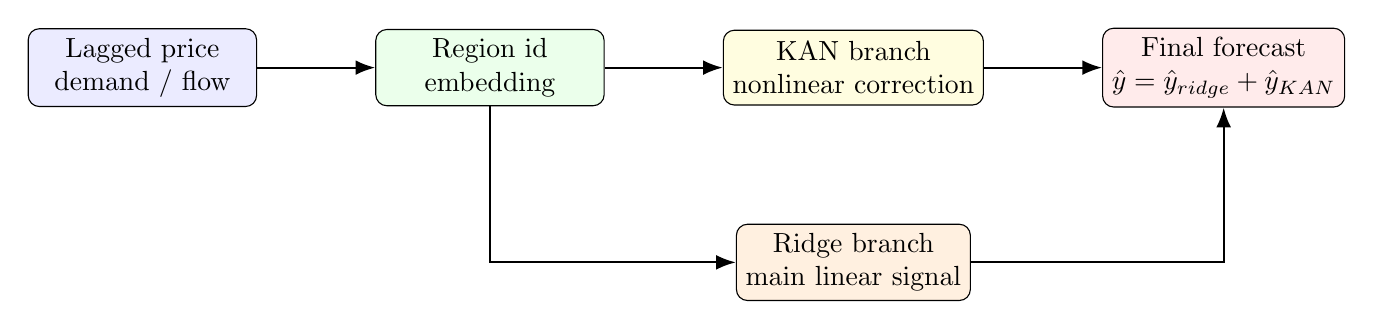
\begin{tikzpicture}[
node distance=1.5cm,
box/.style={draw, rounded corners, align=center, minimum width=2.9cm, minimum height=0.95cm},
arr/.style={-{Latex[length=2.5mm]}, thick}
]
\node[box, fill=blue!8] (lags) {Lagged price\\ demand / flow};
\node[box, fill=green!8, right=of lags] (embed) {Region id\\ embedding};
\node[box, fill=yellow!12, right=of embed] (kan) {KAN branch\\ nonlinear correction};
\node[box, fill=orange!12, below=of kan] (ridge) {Ridge branch\\ main linear signal};
\node[box, fill=red!8, right=of kan] (out) {Final forecast\\ $\hat y = \hat y_{ridge} + \hat y_{KAN}$};
\draw[arr] (lags) -- (embed);
\draw[arr] (embed) -- (kan);
\draw[arr] (embed) |- (ridge);
\draw[arr] (kan) -- (out);
\draw[arr] (ridge) -| (out);
\end{tikzpicture}
\caption{Schematic view of the strengthened electricity forecasting design. The tabular linear branch captures the main signal, while the KAN branch models structured nonlinear corrections conditioned on lagged features and regional context.}
\label{fig:elec_scheme}
\end{figure}

\subsection{Results After Strengthening}

The strengthened setup substantially improved KAN-family performance, as shown in Table~\ref{tab:elec_strong}.

\begin{table}[t]
\centering
\caption{Electricity forecasting: strengthened KAN setup}
\label{tab:elec_strong}
\begin{tabular}{lccc}
\toprule
Model & RMSE & MAE & $R^2$ \\
\midrule
HGBDelta & 102.56 & 55.27 & 0.943 \\
HybridKANEmbedDelta & 107.57 & 61.15 & 0.937 \\
ResidualRidgeKAN & 108.56 & 60.81 & 0.936 \\
KANEmbedDelta & 115.17 & 69.88 & 0.928 \\
RidgeDelta & 116.30 & 69.39 & 0.926 \\
\bottomrule
\end{tabular}
\end{table}

The strongest KAN-based model became HybridKANEmbedDelta with RMSE 107.57, reducing the gap to the best boosting baseline to approximately 5 RMSE points. This is a dramatic improvement compared to the original Hybrid KAN result of RMSE 181.23.

The importance of this result goes beyond the absolute value of the metric. The strengthened KAN models do not merely improve slightly; they recover a large portion of the performance gap created by the naive formulation. This indicates that model quality in applied forecasting depends heavily on how the prediction target, feature representation, and architectural decomposition interact. In this case, the strengthened design makes KAN meaningfully competitive in a regime where its raw version was clearly misaligned with the task.

\subsection{Relative Improvement}

To emphasize the scale of the improvement, Table~\ref{tab:improvement} compares the original and strengthened KAN-family models.

\begin{table}[t]
\centering
\caption{Improvement of KAN-family models on electricity data}
\label{tab:improvement}
\begin{tabular}{lcc}
\toprule
Model family & Original RMSE & Strengthened RMSE \\
\midrule
KAN $\rightarrow$ KANEmbedDelta & 149.51 & 115.17 \\
Hybrid KAN $\rightarrow$ HybridKANEmbedDelta & 181.23 & 107.57 \\
\bottomrule
\end{tabular}
\end{table}

This result is important for the overall narrative of the paper. It shows that KAN's practical value depends strongly on problem formulation. A weak result in a raw setup does not necessarily imply that the architecture itself is unsuitable; rather, it may indicate that the model needs a formulation aligned with its strengths.

Equally importantly, the improvement is interpretable at the modeling level. Each change in the strengthened setup has a concrete rationale, and the combined gain is consistent with those rationales. The better performance is therefore not best understood as accidental hyperparameter luck, but as evidence that KAN can become substantially more effective when its representational role is narrowed and clarified.

\subsection{Interpretability on Electricity Data}

Interpretability remains a major reason to study KAN in the electricity setting. In our experiments, the strongest KAN-related importance patterns consistently involved:
\begin{itemize}
    \item recent price history;
    \item calendar structure such as hour-of-day and cyclical encodings;
    \item load and demand-related history.
\end{itemize}

This is an intuitively plausible result and increases confidence that the model is learning meaningful dynamics rather than relying on purely spurious relationships.

At the same time, it is important to state that interpretability differs between model types. Pure KAN models remain the most directly interpretable. Hybrid KAN models are still useful for interpretation, but only partially so, since the final prediction combines an explicit linear component and a nonlinear KAN component.

Nevertheless, even partial interpretability is valuable. In the strengthened hybrid setting, we can still inspect which inputs dominate the nonlinear correction branch, which channels contribute most to final prediction quality, and whether the learned $\phi$-functions behave in a smooth and plausible way. This is substantially more informative than treating the model as a fully opaque predictor.

From an application perspective, this matters because electricity-market forecasting is often embedded in broader analytical workflows. Researchers and practitioners may want to know not only whether the forecast is accurate, but also whether recent prices, load-related indicators, and calendar variables contribute in a stable and intuitively defensible way. KAN does not solve interpretability completely in this setting, but it does provide a more structured entry point into model inspection than many alternative nonlinear architectures.

\section{Discussion}

\subsection{What We Learned from the Two Cases}

The climate and electricity cases lead to complementary conclusions.

For the climate dataset, Hybrid KAN behaves as a genuinely strong forecasting architecture. The task structure is favorable for KAN: the data form a coherent multivariate sequence, the variables are closely related, and the temporal window formulation aligns well with channel-wise nonlinear transformations.

For the electricity dataset, the situation is different. The task is not simply multivariate sequence prediction; it is panel forecasting with strong cross-sectional heterogeneity and substantial dependence on engineered lag and calendar features. In this regime, tabular baselines such as gradient boosting are naturally very strong. Therefore, it is not surprising that the best overall model is not KAN.

Taken together, the two case studies argue against simplistic claims of the form ``KAN is always better'' or ``KAN is not useful in practice.'' Neither statement is supported by the evidence. The more defensible conclusion is that KAN is highly sensitive to task structure, target design, and the relationship between temporal dynamics and cross-sectional heterogeneity.

That sensitivity should not be viewed only as a weakness. It also suggests that KAN is a model family whose success is strongly linked to thoughtful problem formulation. In research terms, this is valuable because it shifts attention from leaderboard-style comparison toward model-task alignment. A method that reveals such alignment effects can contribute useful methodological insight even when it is not uniformly dominant across all benchmarks.

\subsection{Why KAN Still Matters}

Even though KAN is not the strongest model overall in the electricity case, it remains valuable for several reasons:
\begin{itemize}
    \item it provides structured nonlinear modeling;
    \item it offers more interpretable internal transformations than typical black-box deep models;
    \item with appropriate target design and feature representation, it becomes much more competitive;
    \item it can be integrated into hybrid and residual pipelines rather than used only as a standalone predictor.
\end{itemize}

Thus, KAN should be understood less as a universal winner and more as a model family that is especially useful when interpretability is important and when the problem can be formulated in a way that matches its inductive bias.

This framing is especially productive for thesis-level work. It allows KAN to be positioned neither as hype nor as failure, but as a nuanced modeling tool with identifiable strengths, limitations, and integration points. Such a position is much easier to defend academically than an overly strong claim of universal superiority.

\subsection{Practical Implications}

For practical forecasting projects, the results suggest a useful workflow:
\begin{itemize}
    \item start with strong linear and boosting baselines;
    \item introduce KAN when nonlinear interpretability is important;
    \item prefer hybrid or residual KAN designs over naive direct transfer from unrelated tasks;
    \item pay particular attention to target definition and feature grouping.
\end{itemize}

This workflow is valuable for thesis work and applied research because it frames KAN not as a replacement for all other methods, but as part of a broader model design toolkit.

In practical terms, the paper therefore recommends a staged approach to experimentation. First establish a credible baseline with simple and strong models. Then diagnose whether the remaining error appears likely to contain structured nonlinear signal. Only after that should a more specialized architecture such as KAN be introduced, ideally with a clear interpretability plan and a deliberate feature grouping strategy.

\subsection{Limits of the Current Study}

This work has several limitations.

First, the climate experiments are comparatively smaller and cleaner than the electricity case, which makes direct cross-domain conclusions impossible. Second, the electricity data span a relatively limited time range after applying leakage-safe intersection rules. Third, although the strengthened KAN setup significantly improved results, it did not surpass the best boosting baseline.

Moreover, the study focuses on a specific family of KAN implementations and does not exhaustively cover all possible sequence-oriented KAN designs, attention-based hybrids, or transformer-style variants.

These limitations do not invalidate the findings, but they do bound their scope. The paper should therefore be read as a carefully structured comparative study rather than a final statement about every possible KAN variant. Its main contribution is to identify recurring patterns of success, failure, and improvement under realistic forecasting constraints.

\section{Threats to Validity}

\textbf{Internal validity.} For the electricity case, the main threat was leakage from future information. We explicitly addressed this through lagged daily and monthly features and by forecasting $t+1$ rather than using contemporaneous signals that could encode future knowledge.

\textbf{Construct validity.} RMSE, MAE, and $R^2$ capture predictive quality but do not fully capture operational utility. In some applications, ranking errors, directional errors, or tail-risk performance might matter more.

\textbf{External validity.} The climate and electricity datasets are representative of two practically meaningful settings, but they do not cover all forecasting scenarios. Therefore, the conclusions should be interpreted as evidence about \emph{patterns of applicability} rather than universal claims.

\textbf{Statistical conclusion validity.} The reported results rely on a limited number of benchmark datasets and finite hyperparameter exploration. It is therefore possible that stronger tuning of either KAN or competing baselines would shift some absolute numbers. However, the relative pattern of findings is stable enough to support the main qualitative conclusions.

\section{Conclusion}

This paper presented an extended empirical study of KAN and Hybrid KAN architectures on two forecasting tasks with substantially different structure. On the climate forecasting task, Hybrid KAN achieved the best quality among the tested neural models and demonstrated strong robustness to noisy and incomplete data. On the electricity panel forecasting task, tree-based baselines remained the strongest overall predictors. However, after strengthening the KAN formulation using delta-target prediction, region embeddings, and residual learning, the best KAN-based model approached the strongest baseline much more closely.

The central conclusion is that KAN is most valuable not as a universal forecasting winner, but as an interpretable nonlinear model family whose strengths become particularly visible under appropriate task design. For researchers and practitioners, this means that KAN should be considered both as a predictive model and as an analysis tool for studying nonlinear feature-channel effects in forecasting problems.

More broadly, the study argues for a design-oriented view of forecasting research. The decisive question is often not whether a model class is globally stronger than all alternatives, but whether the data representation, target definition, and architectural decomposition allow that model class to express its strengths. In the climate case, the answer is largely yes. In the electricity case, the answer becomes yes only after the task is reformulated in a way that reduces level effects, represents regional identity more compactly, and assigns nonlinear modeling to a more focused residual role.

Future work includes region-level multi-step electricity forecasting, comparison with standard long-horizon benchmark datasets such as ETT, deeper ablation of basis size and hidden dimensionality, and exploring residual KAN designs on top of strong tree-based baselines. Another promising direction is to connect KAN interpretability more directly with domain validation, for example by systematically comparing learned $\phi$-functions with expert expectations about pollutant interactions or electricity-price response patterns. Such extensions would strengthen the case for KAN not only as a competitive predictor, but also as a useful scientific instrument for structured nonlinear analysis.

\section*{Reproducibility Note}

The study was conducted in a reproducible computational workflow based on Python scripts and Jupyter notebooks. The project includes separate notebooks for exploratory analysis and separate scripts for the baseline leakage-safe electricity experiment and the strengthened KAN experiments. Output artifacts include metric tables, prediction files, and interpretability plots. This structure makes it possible to reuse the study both as a research draft and as a basis for thesis presentation materials.

\bibliographystyle{IEEEtran}
\bibliography{references}

\end{document}
